\documentclass[pdflatex,sn-apa]{sn-jnl}

\usepackage{graphicx}%
\usepackage{multirow}%
\usepackage{amsmath,amssymb,amsfonts}%
\usepackage{booktabs}%
\usepackage{array}%
\usepackage{xcolor}%
\usepackage{enumitem}%

\raggedbottom
\setlength{\textfloatsep}{8pt plus 2pt minus 2pt}
\setlength{\floatsep}{8pt plus 2pt minus 2pt}
\setlength{\intextsep}{8pt plus 2pt minus 2pt}
\makeatletter
\renewcommand\keywords[1]{\gdef\@keywords{\par\addvspace{10pt}{\keywordfont{\bfseries\keywordname:} #1\par}}}
\makeatother

\begin{document}

\title[C-SDVR for Side-Effectful Software Engineering Agents]{C-SDVR: Cost-Aware Runtime Verification and Local Recovery for Side-Effectful Software Engineering Agents}

\author*[1]{\fnm{Anonymous} \sur{Working Copy}}\email{anonymous@example.com}

\affil*[1]{\orgdiv{Author metadata omitted from this working preview}, \orgname{Not for journal upload}, \orgaddress{\country{Metadata pending}}}

\abstract{Software engineering agents edit source files, configuration, build metadata, and repository records, so task completion can coexist with harmful residual changes. We present C-SDVR, a runtime control layer that compares scoped pre/post state, checks executable postconditions, classifies deviation severity, and selects continuation, model-generated local repair, guarded rollback, or safe stop. A controlled benchmark of 240 task templates and 84,000 repeated policy runs isolates the effects of step verification, rollback, and severity gating. To examine autonomous recovery from natural model errors, we sample one initial action for each task--model--repeat tuple and replay it unchanged under five equally scoped policies. The paired Git study comprises 40 tasks, two DeepSeek configurations, three repeats, 240 natural action trajectories, and 1,200 policy executions without post-hoc fault injection. Of 21 initially failing trajectories, nine leave residue. C-SDVR with LLM-generated repair succeeds on 236/240 runs (0.983), preserves state integrity on all 240, repairs 17/21 failures, recovers all 9 residue cases, and safely stops on the remaining four. NoCheck, final replay, and an equally empowered judge-and-repair baseline achieve success/residue rates of 0.913/0.038, 0.946/0.017, and 0.900/0.054, respectively; an oracle repairer reaches 1.000 and is reported as an upper bound. A 192-run repository-scaling study shows snapshot and verification costs grow with repository size, whereas scoped rollback grows primarily with changed-state width. The evidence supports C-SDVR as a bounded verification-to-recovery mechanism for observable, reversible software state, not as a guarantee for open-world or irreversible actions.}

\keywords{automated software engineering; LLM agents; repository agents; software reliability; runtime verification; state-difference verification; local recovery}

\maketitle

\section{Introduction}

LLM agents increasingly act directly on software state. Coding agents inspect repositories, edit source and configuration files, update build metadata, run tests, and coordinate multi-step maintenance work \cite{yang2024sweagent,bouzenia2025repairagent}. This shift changes the reliability problem. A wrong textual answer can often be ignored or regenerated, whereas an incorrect side-effectful action can satisfy a visible target while silently modifying an unrelated file, violating a configuration invariant, or leaving a repository in a partially repaired state.

Benchmarks and repair agents have made parts of this difficulty visible. WebArena and OSWorld expose stateful web and desktop execution \cite{zhou2023webarena,xie2024osworld}; ToolSandbox emphasizes implicit state dependencies in tool use \cite{lu2024toolsandbox}; and OpenComputer argues for verifiable software worlds \cite{wei2026opencomputer}. SWE-agent and RepairAgent demonstrate increasingly autonomous repository navigation and program repair \cite{yang2024sweagent,bouzenia2025repairagent}. SearchSYS and recent work on LLM code review further show both the promise and systematic reliability limits of model-mediated software analysis \cite{dakhama2025searchsys,jin2026codereview}. These systems and benchmarks primarily ask whether a task is solved or a patch is accepted. They do not fully answer a runtime-control question: once a repository-changing step deviates, how should a controller detect the incorrect transition, remove harmful residue, and bound further recovery cost?

This paper studies bounded, reversible operations over files, structured records, and local Git repositories. These settings are narrower than open-world software maintenance, but they expose three properties needed to study recovery rather than only generation. First, expected changes can be expressed as executable postconditions, structured parsers, or tests. Second, deviations can be established from state transitions rather than an agent's self-report. Third, many failures admit a least-change correction: restore an unrelated file, revise one configuration field, or replace a faulty patch without replaying the complete workflow.

We propose C-SDVR, a cost-aware state-difference verification and local recovery framework. It wraps side-effectful actions with scoped snapshots, semantic differences, executable postconditions, severity classification, and guarded recovery. Its novelty is not a new base model or automated program-repair generator. It is the control connection from verifiable state evidence to a bounded decision among continue, local repair, rollback-and-repair, and stop. This connection makes task completion, state integrity, and safe containment separately observable.

The contributions are:
\begin{enumerate}[leftmargin=*]
  \item We define a verifier-to-recovery controller that turns semantic state differences into executable continuation, model-generated local repair, guarded rollback, or safe-stop decisions, with explicit adapter and compensation preconditions.
  \item We separate target satisfaction, harmful residue, integrity-preserving outcome, conditional repair success, and safe containment. The resulting rule policy prefers least-change recovery but makes no optimizer or global-optimality claim.
  \item We conduct a paired repository-agent experiment over 40 local Git tasks, two model configurations, and three repeats. The same 240 naturally generated actions are replayed under five policies, including a judge baseline with equal mutation permissions, yielding 1,200 policy executions and auditable pre/post/final states.
  \item We triangulate the repository evidence with an 84,000-run controlled mechanism benchmark, a 192-run repository-scaling study, executable workflow and browser studies, state-boundary stress tests, and postcondition-quality analyses. Each evidence source is reported with its own denominator and validity boundary.
\end{enumerate}

This paper does not claim to solve general program repair or open-world computer use. It evaluates a reliability-control layer for software environments in which relevant state is observable, postconditions or tests are available, and effects are reversible or explicitly containable.

\subsection{Research Questions}

The study is organized around four research questions.
\textbf{RQ1}: In controlled side-effectful tasks, which outcome changes are attributable to step verification, rollback, and severity gating under matched component capabilities?
\textbf{RQ2}: On paired natural LLM actions over local Git repositories, how does C-SDVR with model-generated repair compare with no checking, final replay, an equally empowered judge-and-repair policy, and an oracle upper bound?
\textbf{RQ3}: What recovery, residue, token, and execution-time trade-offs arise, and how do snapshot, semantic-diff, and rollback costs scale with repository size and changed-state width?
\textbf{RQ4}: How sensitive are the conclusions to postcondition quality, state-scope completeness, snapshot freshness, concurrency, and compensation availability?

\section{Related Work}

Web and computer-use benchmarks such as WebArena, VisualWebArena, OSWorld, WorkArena, ToolSandbox, and OpenComputer have made stateful agent evaluation more realistic by exposing web, desktop, and tool-use environments with observable state \cite{zhou2023webarena,koh2024visualwebarena,xie2024osworld,drouin2024workarena,lu2024toolsandbox,wei2026opencomputer}. Their primary contribution is end-to-end evaluation. This emphasis is consistent with calls to assess agent cost, robustness, and reproducibility alongside accuracy \cite{kapoor2024agents}. C-SDVR instead asks what a runtime controller should do once a scoped side-effectful step deviates.

Judge-based evaluation is another relevant line. MT-Bench, G-Eval, Agent-as-a-Judge, and AgentRewardBench show that LLM judges can assess outputs or trajectories while documenting evaluator biases and benchmark-dependent reliability \cite{zheng2023llmjudge,liu2023geval,zhuge2024agentjudge,lu2025agentrewardbench}. C-SDVR treats judge policies as baselines: a text judge may classify a trajectory, whereas C-SDVR computes executable state differences and uses them to trigger repair or rollback.

The verification component follows the runtime-verification intuition that executions can be monitored against properties during operation \cite{leucker2009runtime,havelund2004javapathexplorer}. The recovery component is related to transaction processing, sagas, classical rollback-recovery protocols, and emerging reversible-agent runtimes, where logs, checkpoints, staged effects, or reversible traces help restore consistent state \cite{gray1992transaction,garciamolina1987sagas,elnozahy2002rollback,fokou2026parallax,chen2026cordon,yu2026shepherd}. Dependability taxonomies distinguish reliability, integrity, and maintainability concerns, while autonomic-computing and Rainbow-style systems connect monitoring to adaptation through explicit control loops \cite{avizienis2004dependability,kephart2003autonomic,garlan2004rainbow}. DeltaBox accelerates whole-sandbox checkpoint/rollback, while Revisable by Design formalizes reversibility and earliest-conflict rollback for mid-execution user revisions \cite{dong2026deltabox,zhai2026revisable}. ACRFence further shows that checkpoint restore can be unsafe when retried external effects acquire new semantics \cite{zheng2026acrfence}. C-SDVR therefore does not claim rollback itself as novel. Its narrower contribution is to connect semantic state-difference evidence to residue-aware, severity- and cost-gated recovery for bounded file/form/workflow effects. It remains complementary to model-mediated reflection, interleaved reasoning and acting, and dynamic replanning \cite{shinn2023reflexion,yao2023react,zhu2026whentoolsfail}.

\begin{table}[htbp]
\centering
\caption{Positioning relative to representative agent and automated-software-engineering work.}
\label{tab:related_compare}
\scriptsize
\setlength{\tabcolsep}{3.0pt}
\begin{tabular}{p{0.20\linewidth}p{0.23\linewidth}p{0.22\linewidth}p{0.27\linewidth}}
\toprule
Work & Primary object & Executable evidence & Recovery role \\
\midrule
Web/desktop benchmarks & End-to-end web or desktop tasks & Environment success checks or verifiable state & Evaluation focus; no recovery-policy comparison \\
Repository agents & Issue resolution and program repair & Tests and repository tools & Generates patches; no residue-aware runtime controller \\
SE analysis systems & Testing and requirement conformance & Tests, artifacts, or review labels & Analysis or recommendations; no state restoration \\
LLM judges & Trajectory assessment & Textual trace and state summaries & Judge feedback or retry; no scoped restoration \\
Recovery runtimes & Containment, staged effects, checkpoints, and traces & Mediated runtime state & Supplies recovery substrate rather than semantic policy selection \\
Revision/replay systems & Revision rollback and replay safety & Action and checkpoint history & Rollback for revision/replay objectives, not post-action residue repair \\
C-SDVR & Repository, file, record, and workflow transitions & Semantic diff, parsers, tests, and pre/post state & Selects continue, local repair, guarded rollback, or stop \\
\bottomrule
\end{tabular}
\end{table}

\subsection{Quality Model and Construct Definition}

C-SDVR is evaluated as a software reliability control layer rather than only as an agent-accuracy technique. Table~\ref{tab:quality_model} relates the study constructs to ISO/IEC 25010:2023 and the dependability taxonomy \cite{iso25010_2023,avizienis2004dependability}. The mapping is interpretive rather than normative: this experiment neither certifies ISO conformance nor measures the complete security, reliability, or maintainability of an agent system. In particular, ``state integrity'' below means preservation of the scoped transition and forbidden-effect constraints. Absence of observed residue is not evidence of confidentiality, authenticity, access control, or complete system integrity.

\begin{table}[htbp]
\centering
\caption{Quality constructs, standards relation, and operational evidence.}
\label{tab:quality_model}
\scriptsize
\setlength{\tabcolsep}{2.8pt}
\begin{tabular}{>{\raggedright\arraybackslash}p{0.17\linewidth}>{\raggedright\arraybackslash}p{0.24\linewidth}>{\raggedright\arraybackslash}p{0.26\linewidth}>{\raggedright\arraybackslash}p{0.22\linewidth}}
\toprule
Study construct & Standards relation & Operational meaning & Primary outcome \\
\midrule
Target correctness & Functional suitability & Intended semantic transition holds & Target satisfaction \\
Operational reliability & Reliability & Outcome under repeated nominal and failing actions & All-run and failure-conditioned success \\
Recoverability & Reliability; recoverability & Failed transition is corrected within bounded scope & Conditional repair and rollback success \\
Scoped state integrity & Security integrity; dependability integrity & No harmful non-gold mutation or unsafe overwrite remains & Residue and integrity-preserving outcome \\
Efficiency & Performance efficiency & Resources consumed by verification and recovery & Time, tokens, actions, bytes \\
Corrective restraint & Study-specific; related to stability & Avoid needless repair under benign differences & Unnecessary repair \\
Auditability & Study-specific; accountability and analyzability & Reconstruct action, evidence, decision, and final state & Raw traces, hashes, versions \\
\bottomrule
\end{tabular}
\end{table}

\section{Problem Formulation}

Let a user task $x$ be decomposed into a sequence of side-effectful steps $S=\{s_1,\ldots,s_n\}$ in an environment $E$. Each step $s_i$ has postconditions $P_i$ over a scoped environment state. C-SDVR records the scoped state immediately before and after the action:
\begin{equation}
  B_i = \operatorname{Snapshot}(E_i^{-}, scope(s_i)), \quad
  A_i = \operatorname{Snapshot}(E_i^{+}, scope(s_i)).
\end{equation}
The state difference is:
\begin{equation}
  \Delta_i = \operatorname{Diff}(B_i, A_i).
\end{equation}
A verifier maps the postconditions, state difference, and post-action state to a deviation set:
\begin{equation}
  D_i = \operatorname{Verify}(P_i, \Delta_i, A_i).
\end{equation}
If $D_i=\emptyset$, the step proceeds. Otherwise, a policy selects a recovery action:
\begin{equation}
  \pi(D_i, R_i, C_i, B) \rightarrow \{\textit{continue}, \textit{repair}, \textit{rollback}, \textit{stop}\},
\end{equation}
where $R_i$ is the estimated risk, $C_i$ is the expected recovery cost, and $B$ is the remaining budget.

The prototype implements a deterministic, lexicographic rule policy rather than solving a learned or numerical optimization problem. It first excludes rollback or repair actions whose snapshot, scope, version, concurrency, or compensation guards fail. Among the remaining actions, it prioritizes lower expected unrecovered harm, then smaller affected-state scope, and finally lower estimated token/action/time cost. Table~\ref{tab:decision} is the complete operational policy used in the experiments. The terms ``cost-aware'' and ``least-change'' therefore describe this ordering and its measured consequences; they do not imply a globally optimal planner.

We report five non-interchangeable outcomes. Target satisfaction checks the requested effect. Harmful residue records a disallowed collateral mutation or forbidden extra effect that remains after execution. For executable code-repair tasks, an incorrect patch confined to an intended path is counted as target failure rather than residue, avoiding double-counting the same defect; changes to non-intended paths remain residue. Task success requires both:
\begin{equation}
  Success = \mathbf{1}[P_{final}(E)] \cdot \mathbf{1}[\neg Residue(E)].
\end{equation}
The study's integrity-preserving outcome is either exact task success or an adapter-approved containment state with no forbidden, unrelated, or newer-state overwrite. In the paired Git study, containment requires restoration to the exact pre-action repository followed by explicit stop. Safe containment is therefore recorded only when task success is false, this clean restoration holds, and the controller stops or escalates. Conditional repair success uses only initially failing trajectories as its denominator and asks whether a triggered repair reaches exact success. These definitions prevent a safe stop from being counted as task completion and prevent visible target completion with residue from being counted as success.

Raw state differences and semantic correctness are kept separate. The verifier can observe whitespace-only formatting changes, but the outcome oracle normalizes such changes for tasks explicitly labeled as semantically benign format noise. Thus, ignoring a cosmetic difference is not counted as failure or residue, whereas changing content, provenance, object identity, or a forbidden field remains harmful.

The formulation assumes that step postconditions are available and correct. This is a deliberate scope boundary rather than a solved subproblem. In many deployed systems, a separate planner or specification extractor would need to translate a natural-language instruction into checkable target objects, expected field values, and forbidden side effects. The experiments therefore test whether state-difference verification and local recovery are useful once such postconditions are present; they do not prove that postconditions can always be inferred correctly from free-form user requests.

\section{C-SDVR Framework}

\subsection{State Snapshotting}

For file and repository operations, the snapshot includes tracked paths, existence, content hashes, and directory membership. Structured JSON, YAML, and TOML files are compared semantically so key reordering is not mislabeled as residue. Code-repair tasks additionally execute visible unit tests and a withheld specification edge check. For web-form operations, the snapshot includes form fields, submission messages, and database records. C-SDVR does not rely on the agent's verbal claim that a step succeeded.

\subsection{Environment-Adapter Contract}

An environment adapter must implement six operations: (1) enumerate the declared scope and capture a restorable snapshot; (2) compute a semantic difference; (3) evaluate target and forbidden-effect postconditions, parsers, or tests; (4) apply a bounded action through an explicit mutation interface; (5) compensate or restore only when the snapshot is fresh and the affected version is unchanged; and (6) emit immutable trace metadata and final-state hashes. The Git adapter exposes structured write, delete, and rename actions inside a temporary repository, rejects path traversal and malformed schemas, ignores version-control metadata and interpreter caches, and distinguishes semantic structured-data equality from byte equality. If scope completeness, freshness, conflict checks, or compensation availability cannot be established, the adapter refuses automatic rollback and returns a stop condition.

\subsection{Deviation Classes and Severity}

We use eight deviation classes. Wrong object, extra side effect, and non-persistence are critical because they can alter out-of-scope state or leave downstream steps relying on a false success claim. Wrong destination, wrong field, wrong content, and partial completion are major target violations that usually remain locally recoverable. Minor format noise is minor only when target semantics are preserved. These are benchmark policy labels, not universal risk categories; formatting with legal or execution consequences must instead be treated as major.

\subsection{Cost-Aware Local Recovery}

C-SDVR estimates risk as a function of goal impact, irreversibility, downstream dependency, and uncertainty. It estimates repair cost using token, time, and action proxies. The policy is:
\begin{enumerate}[leftmargin=*]
  \item continue with logging for low-risk minor deviations;
  \item repair locally when a bounded repair is available and expected benefit exceeds cost;
  \item rollback and then repair when a critical deviation is reversible;
  \item stop or request confirmation when the deviation is critical and not safely reversible.
\end{enumerate}
The severity-restraint component is central. A policy that repairs every detected issue can raise raw success, but it may waste budget and create unnecessary state churn.

\subsection{Algorithmic Procedure}

For each side-effectful step, C-SDVR follows the same bounded control procedure:
\begin{enumerate}[leftmargin=*]
  \item determine the scoped state objects affected by the intended action and record a pre-action snapshot;
  \item execute the agent's proposed action in the file or web-form environment;
  \item record a post-action snapshot and compute the state difference against the pre-action snapshot;
  \item verify the observed difference against the step postconditions and classify any deviation by type and severity;
  \item estimate whether the deviation is ignorable, locally repairable, reversible through rollback, or unsafe to handle automatically;
  \item apply the selected control action: continue, repair the bounded target, rollback then repair, or stop for confirmation;
  \item record the final state hash, success flag, residue flag, recovery action, and cost proxies.
\end{enumerate}
The procedure intentionally separates detection from recovery. The verifier only identifies how the observed state differs from the intended postcondition; the policy layer decides whether spending additional action, time, or token budget is justified.

\begin{table}[htbp]
\centering
\caption{C-SDVR recovery-decision table. The thresholds are policy settings for the bounded experiments rather than universal safety rules.}
\label{tab:decision}
\small
\begin{tabular}{p{0.22\linewidth}p{0.22\linewidth}p{0.42\linewidth}}
\toprule
Verifier outcome & Cost/risk condition & Policy action \\
\midrule
No deviation & Any budget & Continue and log final state hash. \\
Minor formatting deviation & Low downstream risk or high repair cost & Continue with logged warning. \\
Major target deviation & Target object clear and bounded repair available & Repair target locally without replaying prior steps. \\
Critical side effect & Pre-action scoped state available and reversible & Roll back affected scope, then apply bounded repair. \\
Critical or ambiguous side effect & Irreversible, external, or uncertain repair scope & Stop or request confirmation instead of automatic repair. \\
\bottomrule
\end{tabular}
\end{table}

\subsection{Invalid Action and Judge-Failure Handling}

Endpoint-backed validation adds invalid JSON actions, schema or path-boundary violations, and invalid judge outputs. An action that remains unparsable after the configured repair prompts is not executed; its token cost and invalid-action flag are retained, and the unsatisfied postcondition can trigger bounded repair or final replay. Invalid judge JSON is counted separately and treated as uncertainty or failure, never silently as success. If a partially executed command changes state before parsing fails, the observed difference governs recovery; critical or ambiguous changes outside the reversible local scope stop for confirmation. The claims therefore remain restricted to observable, reversible environments.

\subsection{Worked Recovery Trace}

Consider a web-form task: update record \texttt{r1}'s name from ``Alicia'' to ``Alice'' while preserving all other records. Before execution, C-SDVR snapshots the scoped SQLite rows for \texttt{r1} and neighboring records. A wrong-object deviation submits the form for \texttt{r2}; the post-action diff therefore contains two facts: \texttt{r2.name} changed unexpectedly and \texttt{r1.name} remains unsatisfied. The verifier maps this to a critical wrong-object deviation because the target postcondition is false and an unrelated row was modified. Since the prior state is available, the policy first rolls back the \texttt{r2} mutation, then performs a bounded repair by submitting the intended \texttt{r1} update. The final diff contains only the expected \texttt{r1.name} change and no residue. An analogous file trace occurs when a task asks to rename \texttt{draft.txt} but the executor renames \texttt{notes.txt}; C-SDVR restores \texttt{notes.txt} from the pre-action snapshot before retrying the scoped rename.

\begin{figure}[htbp]
\centering
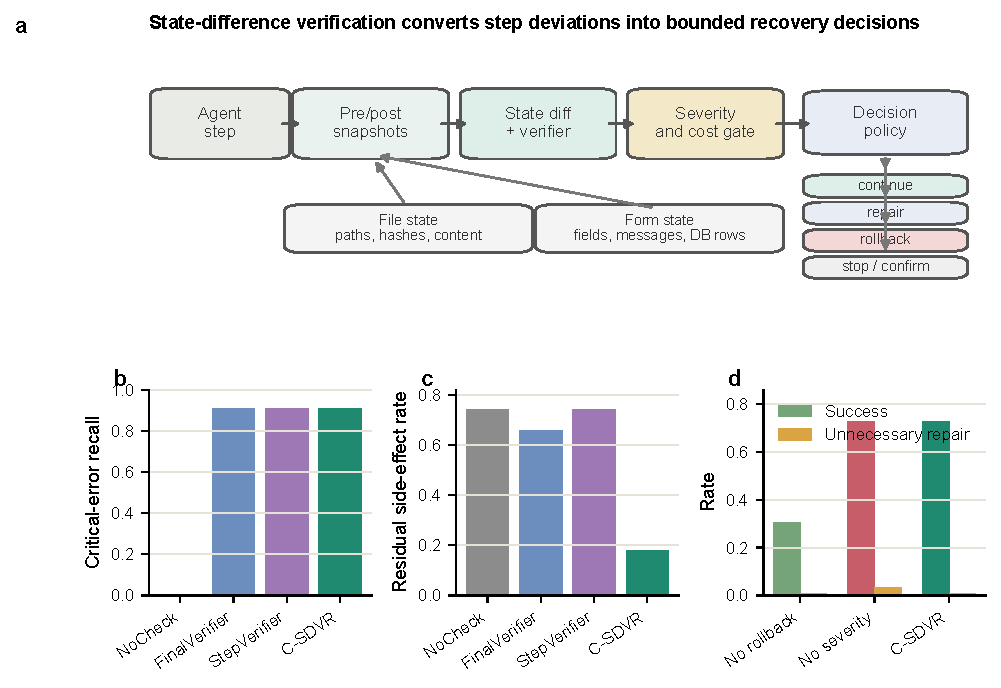
\includegraphics[width=0.96\linewidth]{Fig1.pdf}
\caption{C-SDVR mechanism and immediate evidence. (a) Each side-effectful step is wrapped with pre/post state snapshots, state-difference verification, severity/cost gating, and a bounded decision policy. (b--d) The same mechanism explains the empirical pattern: C-SDVR improves critical-error recall, lowers residual side effects, and uses severity restraint to avoid the unnecessary-repair cost of aggressive recovery.}
\label{fig:framework}
\end{figure}

\section{Study Design}

\subsection{Controlled Mechanism Benchmark}

The first study isolates controller mechanisms under repeatable perturbations. It uses two executable prototype environments. The file environment stores path-content mappings and applies executable operations such as rename, copy, move, delete, edit, create, and batch move. Each action mutates state and each snapshot records path-level content hashes. The web-form environment uses an in-memory SQLite database with records containing identifiers, names, status values, amounts, and notes. Operations include create, edit, status update, delete, amount update, and compound field updates.

\subsection{Tasks and Fault Injection}

The benchmark contains 240 tasks: 120 file tasks and 120 web-form tasks. The tasks cover 13 operation types and eight deviation classes. For every task and seed, one fault draw is generated independently of policy and then reused by all seven policies; the main fault rate is 0.72. This common-random-number design makes policy comparisons genuinely paired. Internal snapshots retain restorable file contents or database rows, while the released logs store pre-action, post-action, and final state hashes.

The execution pipeline has five stages. First, the task generator creates a target operation and structured postconditions. Second, the executor mutates either the file environment or the SQLite-backed form environment. Third, a fault injector applies an operation-compatible deviation. Fourth, the compared policy observes the available state evidence and decides whether to continue, verify only, retry globally, repair locally, or rollback and repair. Fifth, a semantic transition oracle compares the final state with the gold state produced by applying the intended action to the same initial state. Target satisfaction requires every intended change, including file-content provenance, and residue includes every non-gold change that also departs from the initial state. Semantically equivalent whitespace noise is normalized only for the designated minor-format tasks.

\begin{table}[htbp]
\centering
\caption{Deviation classes and severity mapping used in the executable benchmark.}
\label{tab:faults}
\small
\begin{tabular}{p{0.23\linewidth}p{0.16\linewidth}p{0.49\linewidth}}
\toprule
Deviation class & Severity & Examples in file and form tasks \\
\midrule
Wrong object & Critical & Rename the wrong file; update the wrong record identifier. \\
Extra side effect & Critical & Delete or modify an unrelated file; change an unrelated database row. \\
Non-persistence & Critical & Report success without writing the file or committing the form update. \\
Wrong destination & Major & Move a file to the wrong folder; submit a record to the wrong category. \\
Wrong field & Major & Update status instead of amount, or notes instead of name. \\
Wrong content & Major & Write a malformed value or incorrect replacement text. \\
Partial completion & Major & Complete only one item in a multi-file or multi-field operation. \\
Minor format noise & Minor & Benign whitespace, casing, or small formatting differences. \\
\bottomrule
\end{tabular}
\end{table}

\subsection{Compared Policies}

We compare seven policies:
\begin{itemize}[leftmargin=*]
  \item \textbf{NoCheck}: no state verification or repair.
  \item \textbf{FinalVerifier}: verifies only at the end and attempts coarse repair.
  \item \textbf{StepVerifier}: verifies step-level state but performs no repair.
  \item \textbf{ReflectionRetry}: detects failure and performs global retry.
  \item \textbf{C-SDVR-NoRollback}: uses state-difference verification and repair but disables rollback.
  \item \textbf{C-SDVR-NoSeverity}: repairs aggressively without severity restraint.
  \item \textbf{C-SDVR}: full state-difference verification, severity-aware repair, and local rollback.
\end{itemize}

To isolate policy structure from assigned component quality, every verification-capable policy uses the same base detection capability (0.90), and every recovery-capable policy uses the same repair capability (0.78). Rollback-capable variants use the same rollback capability (0.92). These values are deliberately imperfect experimental design points, selected before the corrected run to avoid ceiling performance; they are not fitted estimates of a deployed detector, repairer, or rollback subsystem. The policies differ in observation time, replay scope, rollback availability, and severity gating, not in a hand-assigned detector advantage. In addition to a common scalar perturbation, an independent $4\times4\times4$ grid varies detector, repair, and rollback capability separately over 64 combinations. Closed-scope live and browser recovery uses deterministic scripted oracle functions and is treated as an upper-bound diagnostic rather than empirical calibration of the three design points.

\subsection{Paired Git-Repository Agent Validation}

The primary autonomous-recovery study removes two limitations of the controlled benchmark: injected deviations and scripted repair. It contains 40 synthetic local Git-repository tasks. Thirty tasks cover source maintenance, JSON/YAML/TOML configuration, dependency and build metadata, CI permissions, release synchronization, repository hygiene, and multi-file or rule-based changes. Ten tasks require executable Python repairs for deduplication, Boolean parsing, recursive merge, semantic-version selection, duration parsing, slug generation, secret redaction, chunking, configuration precedence, and dependency ordering. Every code task has visible unit tests and one withheld edge-condition check; structured-data tasks are evaluated by semantic parsers rather than byte equality.

We evaluate two DeepSeek V4 endpoint configurations, three repeats, and 40 tasks, yielding 240 initial trajectories. For each task--model--repeat tuple, the initial action is sampled once at temperature 0.7, executed in a fresh repository, and then replayed unchanged under all five policies. No fault is injected after generation. This pairing ensures that differences arise after the same initial action and post-action state. The action schema permits only bounded write, delete, and rename operations within the temporary repository; path traversal and invalid schemas fail safely.

The five policies are \textsc{NoCheck}; \textsc{FinalReplay}, which restores the pre-state and asks the model to perform the complete task once more after exact final failure; \textsc{JudgeRepair}, which asks the same model to judge the instruction, initial action, before state, post state, and changed paths, then grants one repair call through the same write/delete/rename interface; \textsc{C-SDVR-LLMRepair}, which removes verified unintended changes, supplies structured difference and test evidence, requests one scoped model repair, re-verifies, and restores the initial state before safe stop if repair remains invalid; and \textsc{C-SDVR-OracleUpperBound}, which restores the exact gold state and is not interpreted as an autonomous method. Thus, JudgeRepair and C-SDVR receive equal mutation vocabulary and one repair-generation opportunity; they differ in executable verification, scoped rollback, and recovery evidence.

The study reports final success, target satisfaction, harmful residue, integrity-preserving outcome, safe stop, repair trigger, conditional repair success, repair-induced side effect, judge false success/alarm, tokens, call count, rollback paths/bytes, and invalid JSON. Raw JSONL traces retain instructions, gold state, initial and repair actions, state snapshots, hashes, prompt/oracle versions, and endpoint metadata. Policy contrasts use 10,000 paired task-cluster bootstrap resamples: the six model/repeat observations within each of the 40 tasks are averaged before resampling.

\subsection{Repository Scalability Validation}

We separately measure the adapter rather than mixing local hashing cost with endpoint latency. Synthetic Git repositories cross four tracked-file counts (50, 250, 1,000, and 2,500), two content sizes (1 and 8 KiB per file), three changed-state widths (1, 10, and 50 files), and eight repeats, for 192 runs. Each run measures complete snapshot time and bytes, post-action hash/diff time, semantic verification time, and scoped rollback time; it then asserts an exact clean repository. These are machine-specific engineering measurements, not asymptotic guarantees or measurements of large industrial monorepositories.

\subsection{Judge Baseline Design}

Two judge designs serve different purposes. The earlier v4 endpoint study includes descriptive \textsc{LLMJudgeFinal}, \textsc{LLMJudgeStep}, and \textsc{LLMJudgeRetry} policies that inspect the instruction, action trace, final scoped state, and a structured difference summary; only the retry variant can regenerate a full action. Because that study samples actions independently by policy, it is retained as supplementary compatibility evidence. The paired Git study instead uses \textsc{JudgeRepair}: it sees the shared instruction/action/state evidence and receives the same bounded write/delete/rename vocabulary and one repair call as C-SDVR. Invalid judge JSON is recorded as invalid rather than silently converted to success. This second design is the fair baseline used for the main judge comparison.

\subsection{Metrics}

We report target satisfaction, task success, integrity-preserving outcome, safe containment, detection precision/recall/F1, critical-error recall, conditional repair success, rollback use, unnecessary repair, residual side-effect rate, token-cost proxy, time-cost proxy, action-cost proxy, and cost-normalized success:
\begin{equation}
  CNS = \frac{Success}{Token/2000 + Time/20 + Action/10}.
\end{equation}
This cost-normalized metric is not proposed as a universal benchmark; it is used to compare policies under the same prototype environment. The main benchmark reports both all-run and fault-conditioned success, residue, and token cost, together with fault prevalence. Fault-conditioned outcomes isolate recovery after a deviation, whereas all-run outcomes represent the workload mixture. Live-style and browser efficacy tables are fault-conditioned, but their measured-cost table uses all runs. Endpoint-backed v4 and workflow tables report all-run outcomes. Each table identifies its denominator.

\subsection{Statistical Analysis}

For the controlled benchmark, we report descriptive policy means and paired bootstrap differences against C-SDVR. Pairing uses the shared task, seed, and fault realization. To avoid treating 50 repeats of one task as 50 independent tasks, we first average paired differences within each task and then perform 5,000 task-cluster bootstrap resamples. Success and cost-normalized success are fault-conditioned; token cost uses all paired runs. For the Git study, all five policies share the initial action and post-action state within each trajectory. We first average each paired difference across the two models and three repeats within a task and then use 10,000 bootstrap resamples of the 40 task clusters. The resulting intervals quantify uncertainty across this task set; they do not imply representativeness of industrial repositories.

We run two complementary sensitivity analyses. The first scales detection, repair, and rollback together from 0.80 to 1.20. The second varies them independently over detector $\{0.60,0.75,0.90,1.00\}$, repair $\{0.50,0.65,0.78,0.90\}$, and rollback $\{0.60,0.75,0.92,1.00\}$, with five seeds at each of 64 combinations and deviation-class stratification. This checks interaction effects that a one-dimensional sweep would hide. The supplemental live-style, browser, workflow, boundary, and endpoint-backed validations are reported descriptively because their purpose is external-execution plausibility or failure-boundary analysis rather than population inference.

\subsection{Artifact and Reproducibility Design}

The executable artifact fixes random seeds and records task, domain, method, seed, deviation, target satisfaction, residue, pre/post/final state hashes, verifier and recovery decisions, and cost proxies. It asserts that every injected harmful fault changes the controlled semantic transition and that shared fault realizations do not vary across policies. The Git runner separately asserts five policy replays per trajectory; identical initial-action and post-action hashes; balanced task/model/repeat cells; semantic structured-data comparison; and exact test, hidden-check, and repository-integrity outcomes. Raw CSV, JSONL traces, summaries, paired contrasts, scaling records, and an independent 52-check numeric audit support regeneration. Endpoint metadata and prompt/oracle versions are retained, whereas API keys are never written.

\subsection{Generative AI Assistance and Human Oversight}

Generative AI tools assisted code drafting, debugging, statistical-reporting checks, and manuscript language revision. No generative system is listed as an author. The human author directed the research question and study scope, executed the endpoint-backed experiments, inspected the generated records, audited reported values against source CSV files, and checked bibliographic metadata. The human author remains responsible for the final design, interpretation, manuscript, and submission declarations.

\subsection{Exploratory Language-Variant Audit}

As supplementary construct-validity evidence, two human reviewers independently evaluated 240 synthetic instruction variants using AI-assisted annotation workbooks. They compared the base instruction and variant, reviewed target object, target field, expected state, forbidden-effect set, and meaning preservation, and recorded a decision. This audit does not support the main repository-agent claim and is not treated as an independent user study. The workbook templates retain legacy simulation labels and AI-generation metadata, so reviewer provenance is author-attested rather than independently established by file metadata; source hashes and this limitation are retained in the artifact.

The annotation protocol defines meaning preservation strictly: a variant must retain both the target update and every preservation constraint. We report normalized exact agreement for the four structured fields and percent agreement plus Cohen's $\kappa$ for the binary label. Reviewer uncertainty is not imputed: binary reliability uses the 232 rows on which both reviewers supplied a determinate label. Percentile 95\% intervals use 10,000 task-cluster bootstrap samples over the 80 underlying tasks. After freezing both reviews, the protocol criterion adjudicates only nonmatching rows: an added existence precondition is a semantic change unless present in the base instruction, and two named peers do not preserve a global ``every unrelated object and field'' constraint without an explicit exhaustiveness guarantee.

\subsection{Supplemental Live-Style Validation}

Targeted validations test whether the controlled pattern survives executable boundaries. A 600-run study mutates temporary files and a Flask/SQLite form service; a 300-run Playwright study submits the same form through headless Chromium. Both use policy-shared fault draws and exact gold-state comparison for NoCheck, FinalVerifier, and C-SDVR. Their C-SDVR repair functions are scripted task oracles with complete local scope; perfect recovery therefore measures mechanism execution under an oracle repairer, not autonomous repair synthesis. A separate 180-run endpoint compatibility study uses OpenAI-compatible LLM-generated actions for 10 file and 10 browser-form tasks and evaluates exact final file contents or database rows.

Two further studies address longer and less scripted behavior. A 240-run validation compares NoCheck, FinalVerifier, ReflectionRetry, and C-SDVR on five- or six-step student-record and file-report workflows, with fault sequences shared across policies and rollback scope measured as changed semantic leaves. A 600-run boundary study crosses file and SQLite environments with complete scope, omitted scope, stale snapshots, concurrent modification, and a non-compensable local effect. The legacy v4 endpoint study adds two model configurations, judge baselines, table tasks, and micro-workflow tasks. It executes 40 tasks, six policies, two repeats, and two models (960 policy rows) with the \texttt{semantic-state-v2} oracle. Because each policy receives an independently sampled action and repair remains scripted, v4 is supplementary; the paired Git validation above supersedes it for autonomous-repair and judge comparisons. All retained evidence remains local, reversible, and bounded except for the deliberately non-compensable local boundary surrogate.

\section{Results}

The results are organized by evidence strength and research question. We first report paired natural repository trajectories and autonomous model repair, then use the larger controlled benchmark for mechanism attribution. Scaling, boundary, workflow, and postcondition studies establish cost and validity limits.

\subsection{Paired Natural Repository Trajectories and Autonomous Repair}

The two model configurations generate 240 initial actions, of which 219 satisfy the complete transition and 21 fail naturally. The failures comprise 11 wrong-content patches, nine extra side effects, and one non-persistent action; all nine extra-side-effect trajectories leave harmful residue. Table~\ref{tab:asepaired} compares the five policies on the same initial actions and states. C-SDVR with model-generated repair reaches exact success on 236/240 trajectories (0.983), leaves no residue, and yields an integrity-preserving outcome on all 240. It repairs 17/21 initial failures and removes residue in all 9/9 affected trajectories. The other four failed repair attempts are restored to the clean initial state and explicitly stopped, so they count as failures for task success but successes for containment.

\begin{table}[htbp]
\centering
\caption{Paired Git-repository validation over 240 shared natural trajectories (40 tasks, two model configurations, three repeats; 1,200 policy executions). Conditional repair uses the 21 initially failing trajectories; recovered residue uses the nine initial residue trajectories.}
\label{tab:asepaired}
\scriptsize
\setlength{\tabcolsep}{1.4pt}
\begin{tabular}{lrrrrrrr}
\toprule
Policy & Succ. & Resid. & Integr. & Stop & Repair & R-rec. & Token \\
\midrule
NoCheck & 0.913 & 0.038 & 0.913 & 0.000 & -- & 0/9 & 497.9 \\
FinalReplay & 0.946 & 0.017 & 0.946 & 0.000 & 0.381 & 5/9 & 562.6 \\
JudgeRepair & 0.900 & 0.054 & 0.900 & 0.000 & 0.095 & 1/9 & 1253.0 \\
C-SDVR-LM & \textbf{0.983} & \textbf{0.000} & \textbf{1.000} & 0.017 & \textbf{0.810} & \textbf{9/9} & 578.9 \\
C-SDVR-Oracle & 1.000 & 0.000 & 1.000 & 0.000 & 1.000 & 9/9 & 497.9 \\
\bottomrule
\end{tabular}
\end{table}

Task-cluster paired intervals support the descriptive pattern without treating six model/repeat observations as independent tasks. Relative to NoCheck, C-SDVR increases success by 0.071 (95\% task-cluster bootstrap interval 0.025--0.133), reduces residue by 0.038 (0.008--0.075), and increases integrity-preserving outcomes by 0.088 (0.029--0.158), at 81 additional mean tokens. Relative to JudgeRepair, the corresponding differences are +0.083 success (0.029--0.150), $-0.054$ residue (reduction interval 0.017--0.104), and +0.100 integrity (0.038--0.175), while C-SDVR saves 674 mean tokens (561--800). The success difference from FinalReplay is +0.038 (0.000--0.096), and the oracle upper bound exceeds C-SDVR by 0.017 (0.000--0.046).

The fair judge baseline does not fail merely because it lacks an action interface: it receives one judge call and, when requested, one repair call through the same mutation schema. It nevertheless issues 16 false-success judgments and 20 false alarms, triggers 20 unnecessary repairs, and introduces a new side effect on five trajectories. By contrast, C-SDVR triggers repair only for the 21 executable failures and induces no new side effect. Model stratification shows C-SDVR success/residue of 1.000/0.000 for the flash configuration and 0.967/0.000 for the pro configuration; the latter's four unrepaired tasks account for all safe stops. These bounded results support verification-driven recovery, but the two configurations share one provider and the tasks are synthetic local repositories.

\subsection{Repository-Adapter Scalability}

All 192 scaling runs pass exact semantic verification and clean-repository rollback assertions. Figure~\ref{fig:scalability} separates repository-size cost from changed-state width. With 1 KiB files and ten changed paths, mean snapshot/hash-diff times rise from 6.1/6.0 ms at 50 files to 199.6/199.1 ms at 2,500 files; rollback rises only from 0.43 to 0.64 ms. At 2,500 files, 8 KiB per file, and ten changed paths, the complete snapshot occupies 19.53 MiB and costs 208.2 ms, hash/diff costs 206.9 ms, and scoped rollback costs 0.72 ms. Increasing the changed width to 50 raises rollback to 2.76 ms but has little effect on full snapshot cost. The current adapter therefore scales approximately with total tracked content for complete snapshots and with changed-state width for rollback; incremental or VCS-native snapshots are needed for substantially larger repositories.

\begin{figure}[htbp]
\centering
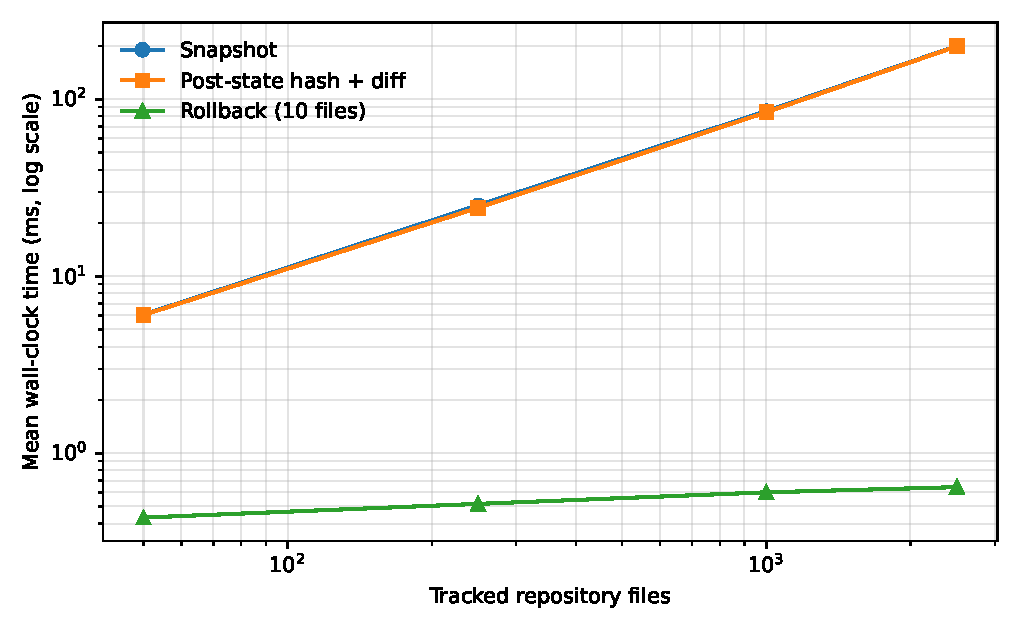
\includegraphics[width=0.96\linewidth]{Fig6.pdf}
\caption{Repository-adapter scaling over 192 exact-state runs. Snapshot and hash/diff cost grow with tracked repository size and content volume, whereas scoped rollback is driven primarily by the number of changed paths. Values are machine-specific means over eight repeats per design cell.}
\label{fig:scalability}
\end{figure}

\subsection{Controlled Mechanism Results}

Table~\ref{tab:main} summarizes the paired benchmark. C-SDVR recovers 0.727 of fault-conditioned runs, compared with 0.125 for NoCheck, 0.303 for FinalVerifier, and 0.125 for StepVerifier. It reduces fault-conditioned residual side effects from 0.742 under NoCheck and 0.657 under FinalVerifier to 0.180. ReflectionRetry has 0.017 higher success, but leaves more residue (0.216 versus 0.180) and uses 56\% more all-run token-cost proxy (3178.4 versus 2039.9). C-SDVR-NoSeverity matches C-SDVR's success and residue but incurs more token cost and unnecessary repair. Thus, C-SDVR is not the raw-success optimum; it is the strongest tested residue--cost compromise under the reported cost profiles.

\begin{table}[htbp]
\centering
\caption{Main executable-state benchmark results. Fault success, residue, detection metrics, rollback use, and CNS are conditioned on an injected deviation; token cost and unnecessary repair use all 84,000 runs.}
\label{tab:main}
\scriptsize
\setlength{\tabcolsep}{2.5pt}
\begin{tabular}{lrrrrrrr}
\toprule
Method & F. succ. & F1 & Crit. & F. resid. & Token & Unnec. & CNS \\
\midrule
NoCheck & 0.125 & 0.000 & 0.000 & 0.742 & 947.0 & 0.000 & 0.108 \\
FinalVerifier & 0.303 & 0.914 & 0.907 & 0.657 & 2116.3 & 0.034 & 0.130 \\
StepVerifier & 0.125 & 0.914 & 0.907 & 0.742 & 1416.7 & 0.000 & 0.083 \\
ReflectionRetry & \textbf{0.744} & 0.914 & 0.907 & 0.216 & 3178.4 & 0.034 & 0.200 \\
C-SDVR-NoRollback & 0.305 & 0.914 & 0.907 & 0.655 & 1959.9 & 0.009 & 0.148 \\
C-SDVR-NoSeverity & 0.727 & 0.914 & 0.907 & \textbf{0.180} & 2210.6 & 0.034 & 0.290 \\
C-SDVR & 0.727 & \textbf{0.914} & \textbf{0.907} & \textbf{0.180} & 2039.9 & \textbf{0.009} & \textbf{0.309} \\
\bottomrule
\end{tabular}
\end{table}

The shared fault prevalence is 0.725 (8697 of 12,000 runs per policy). Table~\ref{tab:denominators} prevents recovery efficacy from being conflated with nominal no-fault performance. C-SDVR's all-run success is 0.802, compared with 0.727 after conditioning on a fault; its mean token-cost proxy rises from 1624.4 on nominal runs to 2197.7 on faulted runs. All policies achieve the intended state on the nominal stratum, so policy differences arise from recovery behavior and its overhead.

\begin{table}[htbp]
\centering
\caption{All-run and fault-conditioned denominators. Each policy has 12,000 all runs and 8,697 faulted runs; fault prevalence is 0.725.}
\label{tab:denominators}
\scriptsize
\setlength{\tabcolsep}{2.8pt}
\begin{tabular}{lrrrrrr}
\toprule
Method & All succ. & Fault succ. & All resid. & Fault resid. & Token all & Token fault \\
\midrule
NoCheck & 0.366 & 0.125 & 0.538 & 0.742 & 947.0 & 948.0 \\
FinalVerifier & 0.495 & 0.303 & 0.476 & 0.657 & 2116.3 & 2348.8 \\
StepVerifier & 0.366 & 0.125 & 0.538 & 0.742 & 1416.7 & 1459.3 \\
ReflectionRetry & \textbf{0.814} & \textbf{0.744} & 0.157 & 0.216 & 3178.4 & 3510.3 \\
C-SDVR-NoRollback & 0.496 & 0.305 & 0.475 & 0.655 & 1959.9 & 2117.7 \\
C-SDVR-NoSeverity & 0.802 & 0.727 & \textbf{0.130} & \textbf{0.180} & 2210.6 & 2372.5 \\
C-SDVR & 0.802 & 0.727 & \textbf{0.130} & \textbf{0.180} & 2039.9 & 2197.7 \\
\bottomrule
\end{tabular}
\end{table}

\begin{figure}[htbp]
\centering
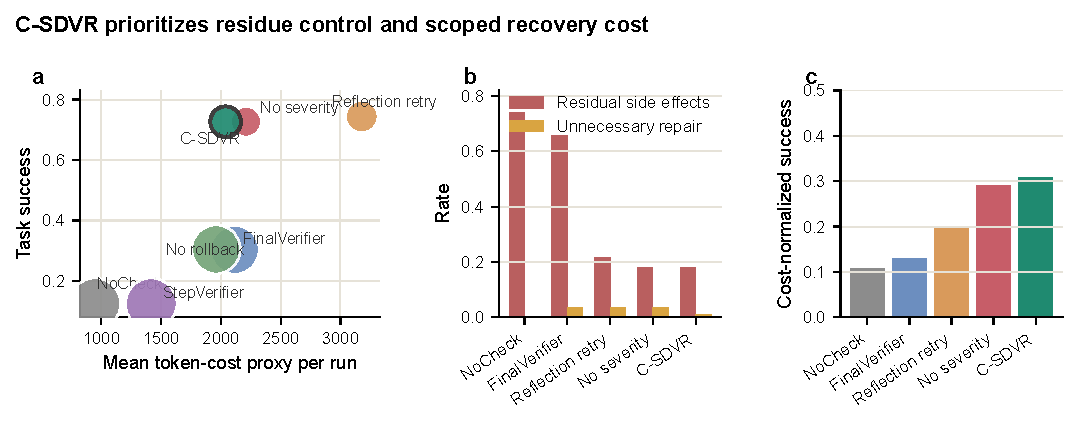
\includegraphics[width=0.96\linewidth]{Fig2.pdf}
\caption{Main trade-off across policies. (a) ReflectionRetry has slightly higher fault-conditioned success, whereas C-SDVR uses less recovery cost and leaves less residue; marker size encodes residue. (b) Rollback lowers residual side effects, and severity restraint reduces unnecessary repair. (c) C-SDVR has the highest cost-normalized success under the stated proxy.}
\label{fig:tradeoff}
\end{figure}

\subsection{Does Step-Level Verification Suffice?}

StepVerifier reaches the same detection quality as the recovery policies (F1 0.914; critical recall 0.907), but its success remains 0.125, identical to NoCheck. Detection alone therefore does not restore state; the verifier must be connected to a recovery action.

\subsection{Does Local Rollback Matter?}

C-SDVR outperforms C-SDVR-NoRollback in success (0.727 vs. 0.305), residual side-effect reduction (0.180 vs. 0.655), and cost-normalized success (0.309 vs. 0.148). The difference is concentrated in critical deviations: C-SDVR reaches 0.668 success and 0.135 residue, whereas the rollback-disabled policy reaches 0.151 and 0.795. Among rollback attempts, the operation succeeds on 0.915 of runs. When rollback fails, the corrected implementation no longer restores the exact gold state through an implicit fallback; the remaining target-only repair can therefore leave critical residue. Rollback changes the recoverable state rather than merely the log, but it is not assumed infallible.

\subsection{The Cost of Aggressive Repair}

C-SDVR-NoSeverity and C-SDVR have the same success (0.727) and residue (0.180), but the aggressive policy uses a higher token-cost proxy (2210.6 vs. 2039.9) and triggers nearly four times as many unnecessary repairs (0.034 vs. 0.009). On minor-format tasks, both preserve semantic success, while C-SDVR avoids most cosmetic repair. Severity restraint is therefore supported as an efficiency mechanism, not as a way to trade away genuine correctness.

The matched-capability result removes the earlier ambiguity in which NoSeverity bought higher success through more aggressive repair. Here, NoSeverity is dominated by C-SDVR on token cost and unnecessary repair while tying it on success and residue. ReflectionRetry instead has slightly higher success (0.744) but leaves more residue (0.216) and uses substantially more token-cost proxy (3178.4). These comparisons support the least-change interpretation within the controlled environment; they do not prove universal deployment optimality.

\subsection{Safety Metrics}

Figure~\ref{fig:safety} shows that C-SDVR has the strongest combination of critical-error recall and low residual side effects. FinalVerifier and ReflectionRetry detect some failures, but their late detection makes local recovery less effective and more expensive. The domain-level view further shows that file tasks remain harder than web-form tasks because file operations include more path-level and content-level side effects; nevertheless, rollback reduces residual harm in both domains.

\begin{figure}[htbp]
\centering
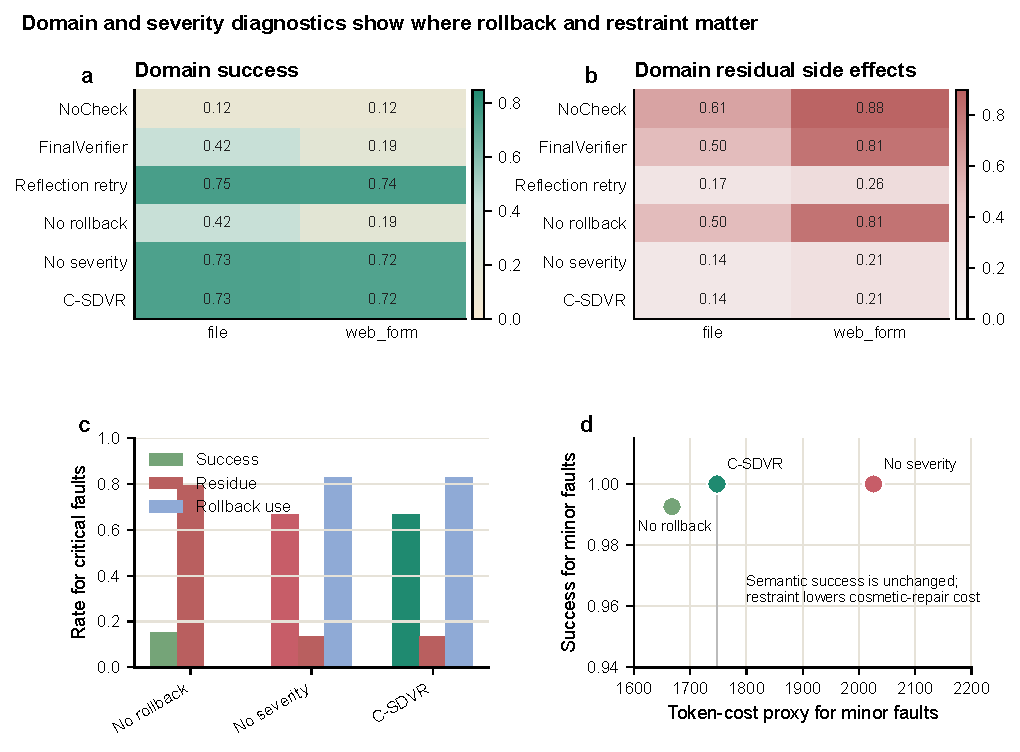
\includegraphics[width=0.96\linewidth]{Fig3.pdf}
\caption{Domain and severity diagnostics. (a,b) C-SDVR reduces residual side effects in both domains. (c) Rollback distinguishes C-SDVR from the rollback-disabled ablation on critical deviations. (d) Minor formatting differences remain semantically successful, while severity restraint avoids cosmetic repair cost.}
\label{fig:safety}
\end{figure}

\subsection{Bootstrap Differences and Sensitivity}

Task-cluster bootstrap differences show that C-SDVR improves fault-conditioned success over NoCheck by 0.602, over FinalVerifier by 0.426, and over C-SDVR-NoRollback by 0.424. ReflectionRetry is higher by 0.017, while C-SDVR gains 0.109 cost-normalized success and saves about 1,139 token-cost units. C-SDVR ties C-SDVR-NoSeverity in success while gaining 0.019 cost-normalized success and saving 171 token-cost units. Common scaling from 0.80 to 1.20 raises C-SDVR success from 0.509 to 0.931 and cost-normalized success from 0.223 to 0.390.

\begin{table}[htbp]
\centering
\caption{Bootstrap paired differences against C-SDVR in the main benchmark. Positive success and CNS differences mean C-SDVR is higher; positive token differences mean C-SDVR uses more token-cost proxy. Intervals are percentile 95\% bootstrap intervals.}
\label{tab:bootstrap}
\small
\setlength{\tabcolsep}{2.8pt}
\begin{tabular}{lrrr}
\toprule
Comparator & Success diff & CNS diff & Token diff \\
\midrule
NoCheck & 0.602 [0.570, 0.632] & 0.201 [0.174, 0.225] & 1092.9 [1073.6, 1111.8] \\
FinalVerifier & 0.426 [0.384, 0.466] & 0.180 [0.164, 0.195] & -76.4 [-85.5, -67.5] \\
StepVerifier & 0.602 [0.571, 0.631] & 0.226 [0.209, 0.243] & 623.2 [606.9, 639.1] \\
ReflectionRetry & -0.017 [-0.021, -0.013] & 0.109 [0.104, 0.115] & -1138.5 [-1152.3, -1124.2] \\
C-SDVR-NoRollback & 0.424 [0.381, 0.466] & 0.162 [0.145, 0.179] & 80.0 [80.0, 80.0] \\
C-SDVR-NoSeverity & 0.000 [0.000, 0.000] & 0.019 [0.017, 0.021] & -170.7 [-174.8, -167.0] \\
\bottomrule
\end{tabular}
\end{table}

The independent capability grid in Figure~\ref{fig:capability} separates detector, repair, and rollback effects. At the design point $(0.90,0.78,0.92)$, five-seed fault-conditioned success is 0.726 and residue is 0.184. Across all 64 combinations, detector and repair capability jointly determine whether a deviation reaches a successful corrective action; rollback capability primarily changes critical wrong-object, extra-effect, and non-persistence outcomes. The full deviation-class grid is supplied as machine-readable data. The monotone surface shows that the headline result is not created by one scalar multiplier, while also confirming that performance degrades substantially when any component is weak.

\begin{figure}[htbp]
\centering
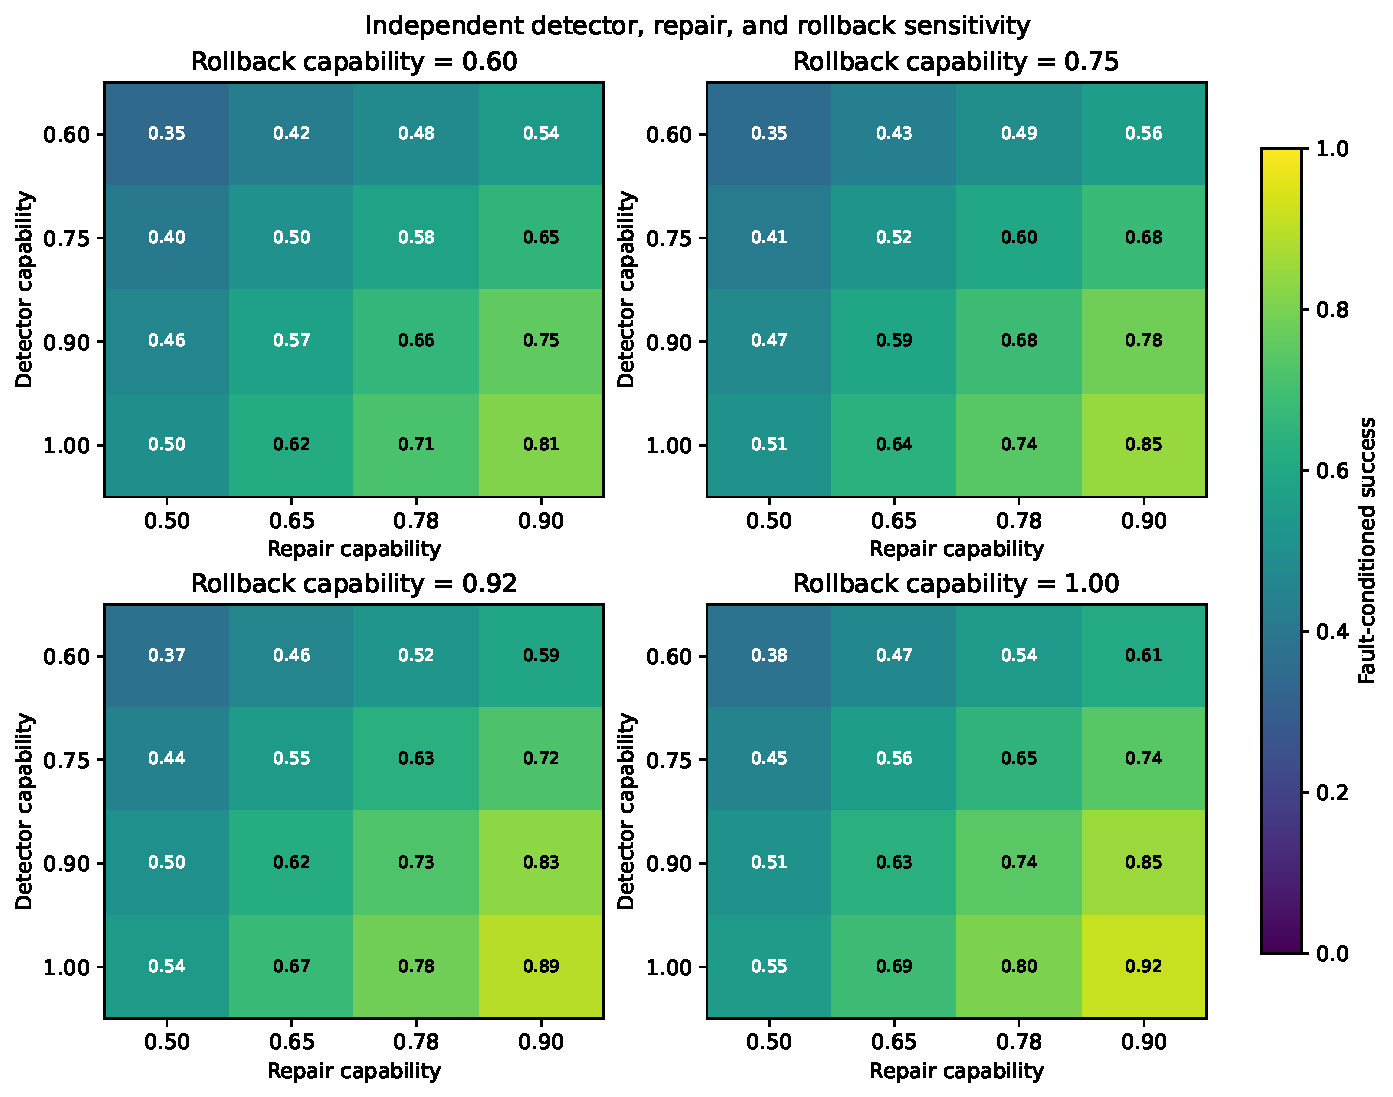
\includegraphics[width=0.94\linewidth]{Fig5.pdf}
\caption{Independent $4\times4\times4$ detector--repair--rollback capability grid. Each panel fixes rollback capability; rows vary detector capability and columns vary repair capability. Cell values are fault-conditioned C-SDVR success averaged over five seeds. The parameters are experimental design points, not fitted deployment estimates.}
\label{fig:capability}
\end{figure}

\subsection{Fault-Rate, Cost-Weight, and Postcondition Robustness}

Because the main benchmark uses a controlled fault rate and a hand-specified cost-normalized-success denominator, we added reviewer-requested robustness analyses. When the controlled fault rate changes from 0.20 to 0.80, C-SDVR success ranges from 0.712 to 0.741, residual side effects from 0.177 to 0.190, and cost-normalized success from 0.303 to 0.316. C-SDVR and the no-severity ablation retain the same success and residue at each tested rate, while severity gating lowers token cost and unnecessary repair. The result supports an efficiency interpretation rather than a universal-best-policy claim.

We also re-score the main raw logs under five base, token-heavy, action-heavy, safety-heavy, and success-heavy profiles. C-SDVR ranks first and C-SDVR-NoSeverity second under every tested profile. This stability follows from their tied success and residue together with C-SDVR's lower token and unnecessary-repair costs. Cost-normalized success remains a diagnostic lens, not a substitute for reporting success, residue, unnecessary repair, and token cost separately.

Figure~\ref{fig:pareto} makes this trade-off explicit. ReflectionRetry remains on the Pareto frontier because its success is 0.017 higher, but it uses 56\% more token-cost proxy and has 0.037 higher residue than C-SDVR. C-SDVR dominates C-SDVR-NoSeverity because their success and residue are equal while C-SDVR uses less token cost and fewer unnecessary repairs. NoCheck is cheap but lies outside the residue-constrained region. The intended interpretation is conditional: C-SDVR ranks first under all five tested weighted profiles and is the lowest-cost member of the lowest-residue high-success group, not a universal optimum for arbitrary agents or cost models.

\begin{figure}[htbp]
\centering
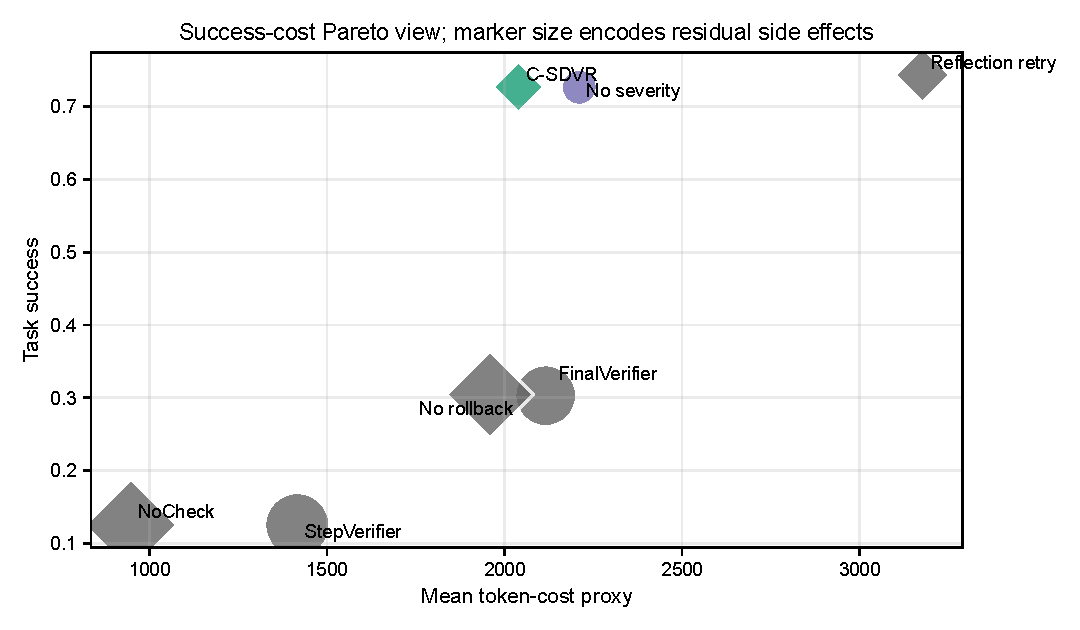
\includegraphics[width=0.92\linewidth]{Fig4.pdf}
\caption{Success-cost Pareto view. The horizontal axis is mean token-cost proxy and the vertical axis is fault-conditioned task success. Marker size encodes residual side-effect rate. ReflectionRetry trades greater cost and residue for 0.017 higher success; C-SDVR provides the best tested weighted residue--cost compromise.}
\label{fig:pareto}
\end{figure}

Finally, we run a controlled postcondition-robustness proxy. This analysis perturbs the verifier-side postcondition to estimate sensitivity to common specification errors, and is complemented below by an endpoint-backed LLM-generated postcondition study. Table~\ref{tab:pcrobust} shows that target-only postconditions reduce success from 0.635 to 0.497 and raise residue from 0.266 to 0.431. Under-specification lowers success further to 0.352, while a wrong-object specification lowers success to 0.153 and raises residue to 0.763. Over-strict constraints slightly increase measured success in this simulator but trigger unnecessary repair on 0.100 of runs, illustrating that one scalar outcome cannot diagnose specification quality. Local recovery therefore depends materially on correct target and forbidden-side-effect clauses.

\begin{table}[htbp]
\centering
\caption{Postcondition robustness proxy for C-SDVR. Gold postconditions are compared with controlled verifier-side postcondition perturbations; endpoint-backed generated postconditions are evaluated separately in Table~\ref{tab:pcgen}.}
\label{tab:pcrobust}
\small
\begin{tabular}{lrrrrrr}
\toprule
PC mode & Success & Target sat. & Residue & F1 & Unnec. repair & Token \\
\midrule
Gold PC & 0.635 & 0.722 & 0.266 & 0.912 & 0.008 & 2035.5 \\
Target-only PC & 0.497 & 0.749 & 0.431 & 0.781 & 0.004 & 1936.7 \\
Under-specified PC & 0.352 & 0.512 & 0.532 & 0.628 & 0.004 & 1850.5 \\
Over-strict PC & 0.657 & 0.733 & 0.244 & 0.871 & 0.100 & 2097.0 \\
Wrong-object PC & 0.153 & 0.239 & 0.763 & 0.705 & 0.172 & 2067.8 \\
\bottomrule
\end{tabular}
\end{table}

\subsection{Supplemental Live-Style Validation Results}

Table~\ref{tab:live} reports fault-conditioned outcomes: C-SDVR reaches 1.000 success with zero residue, whereas FinalVerifier reaches 0.324 success and 0.676 residue. C-SDVR is 1.000 in every observed file and form deviation class (10 strata, 11--18 faulted runs per stratum), including wrong object, extra side effect, non-persistence, wrong content or destination, and partial completion. This ceiling follows from complete local scope and a deterministic scripted repair oracle; it demonstrates that the verification-to-recovery plumbing executes correctly, not that an LLM can synthesize perfect repairs. A 180-run exact-state endpoint check yields 0.933--1.000 success across the three policies; few natural errors limit it to compatibility evidence.

\begin{table}[htbp]
\centering
\caption{Supplemental live-style validation using real temporary filesystem operations and a local Flask/SQLite HTTP form service. C-SDVR uses a scripted repair oracle with complete local scope.}
\label{tab:live}
\small
\begin{tabular}{lrrrrrr}
\toprule
Method & Success & Residue & Detection F1 & Crit. rec. & Token & CNS \\
\midrule
NoCheck & 0.000 & 0.777 & 0.000 & 0.000 & 700.0 & 0.000 \\
FinalVerifier & 0.324 & 0.676 & \textbf{1.000} & \textbf{1.000} & 2086.2 & 0.141 \\
C-SDVR & \textbf{1.000} & \textbf{0.000} & \textbf{1.000} & \textbf{1.000} & 2064.2 & \textbf{0.454} \\
\bottomrule
\end{tabular}
\end{table}

\subsection{Browser-Based Web-Form Validation}

Chromium loads, fills, and submits a local HTML form, after which the verifier compares SQLite state with an exact gold transition. Table~\ref{tab:browser} reports fault-conditioned success and residue while retaining no-fault runs for cost and unnecessary-repair accounting. C-SDVR restores the gold state in each of five observed deviation classes (10--16 faulted runs per class); FinalVerifier reaches 0.362 because target replay cannot remove every wrong-object or extra-side-effect mutation without scoped rollback. As in the live study, the repair action is a scripted oracle with complete scope. This supports bounded browser execution and instrumented state restoration, not open-world generalization or autonomous repair synthesis.

\begin{table}[htbp]
\centering
\caption{Browser-based validation using headless Chromium, Playwright, a local Flask HTML form, and SQLite state. Success and residue are fault-conditioned; C-SDVR uses a scripted repair oracle.}
\label{tab:browser}
\small
\begin{tabular}{lrrrrrr}
\toprule
Method & Fault succ. & Fault residue & Detection F1 & Crit. rec. & Token & CNS \\
\midrule
NoCheck & 0.000 & 0.783 & 0.000 & 0.000 & 720.0 & 0.000 \\
FinalVerifier & 0.362 & 0.638 & \textbf{1.000} & \textbf{1.000} & 2127.3 & 0.148 \\
C-SDVR & \textbf{1.000} & \textbf{0.000} & \textbf{1.000} & \textbf{1.000} & 2124.1 & \textbf{0.424} \\
\bottomrule
\end{tabular}
\end{table}

\subsection{Measured Local Execution Costs}

Table~\ref{tab:measured_costs} supplements the normalized proxy with directly measured wall-clock time and serialized state volume. On the instrumented machine, browser execution dominates latency (approximately 0.78--0.80 s per run), while filesystem and local SQLite operations complete in approximately 4 and 37 ms. C-SDVR snapshots are 94--183 bytes in these deliberately small scopes, and a used rollback restores 39--63 bytes on average. These values are implementation- and machine-specific; they exclude external API billing, network variability, and human confirmation time. CNS remains a controlled comparison proxy, not a substitute for these physical measurements.

\begin{table}[htbp]
\centering
\caption{Measured all-run execution costs in the local validations. Rollback bytes are conditional on local rollback use; FinalVerifier performs full target replay rather than scoped rollback.}
\label{tab:measured_costs}
\scriptsize
\setlength{\tabcolsep}{3.2pt}
\begin{tabular}{llrrrr}
\toprule
Environment & Method & Mean ms & P95 ms & Snapshot B & Rollback B \\
\midrule
Temporary file & FinalVerifier & 3.50 & 4.57 & 94 & 0.00 \\
Temporary file & C-SDVR & 3.78 & 5.35 & 94 & 63.03 \\
HTTP/SQLite form & FinalVerifier & 36.40 & 41.20 & 183 & 0.00 \\
HTTP/SQLite form & C-SDVR & 37.50 & 41.13 & 183 & 38.62 \\
Chromium/SQLite & FinalVerifier & 802.36 & 896.05 & 183 & 0.00 \\
Chromium/SQLite & C-SDVR & 783.92 & 869.04 & 183 & 41.07 \\
\bottomrule
\end{tabular}
\end{table}

\subsection{Multi-Step Side-Effectful Workflow Validation}

Table~\ref{tab:workflow} reports the bounded multi-step workflow validation. NoCheck and ReflectionRetry leave substantial final residue once several side-effectful steps interact. FinalVerifier reaches 1.000 success by replaying the full workflow after final failure detection, but uses a higher token-cost proxy than C-SDVR. C-SDVR also reaches 1.000 success and zero final residue while repairing at the detected step; its mean rollback scope is 3.10 changed semantic leaves. Its advantage here is not higher final correctness than the strong full-replay oracle, but comparable correctness with lower scoped recovery cost and an explicit rollback-depth record.

\begin{table}[htbp]
\centering
\caption{Multi-step side-effectful workflow validation over student-record and file-report workflows. Each workflow contains five or six local side-effectful steps.}
\label{tab:workflow}
\small
\setlength{\tabcolsep}{3.2pt}
\begin{tabular}{lrrrrrrr}
\toprule
Method & Runs & Success & Final residue & Interm. residue & Repair & Rollback & Token \\
\midrule
NoCheck & 60 & 0.050 & 0.850 & 2.22 & 0.00 & 0.00 & 600.0 \\
FinalVerifier & 60 & \textbf{1.000} & \textbf{0.000} & 2.22 & 0.95 & 0.00 & 2275.0 \\
ReflectionRetry & 60 & 0.383 & 0.517 & 2.22 & 0.00 & 0.00 & 2595.0 \\
C-SDVR & 60 & \textbf{1.000} & \textbf{0.000} & 2.15 & 2.15 & 2.15 & \textbf{1718.0} \\
\bottomrule
\end{tabular}
\end{table}

The workflow case study clarifies the baseline assumptions. In the student-record workflow, an extra-side-effect update changes an unrelated student status, a wrong-field update violates the target field, and a non-persistence error prevents export generation. C-SDVR detects each deviation immediately, restores only the pre-step scoped state, and repairs the intended target. FinalVerifier is intentionally strong: it detects the failure only at workflow end, restores the initial workflow snapshot, and replays all six steps from a clean plan. This comparison therefore favors FinalVerifier more than many real deployments would, because it assumes a complete clean snapshot and replayable plan; even under that strong baseline, C-SDVR matches final correctness with lower token-cost proxy.

\subsection{Legacy Endpoint Compatibility Check}

The earlier v4 endpoint study uses two endpoint configurations, anonymized as Model-A and Model-B, on 40 bounded tasks, six policies, and two repeats, producing 960 policy rows and 480 judge records. The \texttt{semantic-state-v2} oracle verifies file content provenance and every requested structured field. All action and judge outputs are valid JSON, and the retained trace contains raw/parsed actions, complete scoped states, state hashes, recovery decisions, endpoint metadata, and latency.

C-SDVR and the strong clean-replay FinalVerifier both reach 1.000 success, compared with 0.963 for NoCheck. Judge-policy success ranges from 0.931 to 0.981 while consuming about twice the endpoint tokens of C-SDVR. C-SDVR and FinalVerifier have nearly identical mean token use (1035.9 versus 1035.4), so this experiment does not establish a cost advantage over replay. All 40 target failures occur in one micro-workflow schema and no action leaves residue. Because policies receive independent model samples, this check supports endpoint compatibility and motivates the stronger paired Git design; detailed per-policy data remain in the supplementary artifact rather than serving as principal evidence.

\subsection{LLM-Generated Postcondition Study}

Each endpoint configuration generates 80 postconditions covering v4 and benchmark-derived tasks. We score target object, field, constraint, and forbidden-side-effect clauses against gold specifications, then execute paired mutable-state replays under Gold-PC, LLM-PC, and a deliberately wrong-target PC. The same task, seed, and agent error are reused across PC modes; success requires the exact gold state, and residue is computed from the final semantic state. The task language is constrained and templated, so this is not evidence that arbitrary instructions can be specified correctly.

Table~\ref{tab:pcgen} reports 1.000 on all four generation components for Model-A and 0.988 for Model-B, whose invalid-JSON rate is 0.013. LLM-PC downstream success is correspondingly 1.000 and 0.988, with residue 0.000 and 0.013. The wrong-target PC yields zero success and residue 1.000 for both configurations; it also triggers false and unnecessary repair on 0.150 and 0.238 of Model-A and Model-B runs. Postcondition quality is therefore a material dependency rather than a theoretical caveat.

\begin{table}[htbp]
\centering
\caption{Endpoint-backed LLM-generated postconditions and executable downstream validation. Generation accuracy summarizes object, field, constraint, and forbidden-side-effect correctness. Gold-PC success is 1.000 for both anonymized configurations. Generation has 80 items per configuration; each downstream PC mode has 400 paired state replays per configuration.}
\label{tab:pcgen}
\scriptsize
\setlength{\tabcolsep}{2.2pt}
\begin{tabular}{lrrrrrr}
\toprule
Model & Gen. acc. & Invalid & LLM succ. & LLM resid. & Wrong succ. & Wrong resid. \\
\midrule
Model-A & 1.000 & 0.000 & 1.000 & 0.000 & 0.000 & 1.000 \\
Model-B & 0.988 & 0.013 & 0.988 & 0.013 & 0.000 & 1.000 \\
\bottomrule
\end{tabular}
\end{table}

To test less templated language, we further generate postconditions for 240 natural-language variants per model (480 generations). The variants cover pronoun coreference, conditionals with negative preservation constraints, and elliptical instructions that name two objects to keep unchanged. Human review shows that this set is not a pure paraphrase benchmark: 80 pronoun-coreference variants preserve the base meaning, whereas all 80 conditional and all 80 elliptical variants alter a precondition or preservation scope under the protocol's strict instruction-level criterion. Table~\ref{tab:pcnatural} therefore reports an extraction stress test against canonical executable fields and explicit preservation clauses, not performance on 240 semantically equivalent inputs.

All 480 responses are valid JSON. Both models resolve pronoun targets and values accurately, but preservation recall is only 0.400 and 0.344. Elliptical instructions preserve the two named peer objects (recall 1.000) while target-object, field, and value accuracy falls to approximately 0.76--0.79. Conditional instructions reveal model-specific object/field errors and preservation omissions. Strict representation-level agreement between the two models is 0.946 for object, 0.950 for field, 0.704 for expected state, 0.312 for forbidden effects, and 0.150 for the entire JSON object. These automated component scores remain descriptive because two-thirds of the retained variants intentionally expose semantic shifts rather than equivalence-preserving paraphrase robustness.

\begin{table}[htbp]
\centering
\caption{Natural-language postcondition generation by linguistic phenomenon (80 instructions per model and phenomenon; 480 generations total). Forbidden denotes recall of required preservation clauses. Invalid JSON is 0.000 in every stratum.}
\label{tab:pcnatural}
\scriptsize
\setlength{\tabcolsep}{4.0pt}
\begin{tabular}{llrrrr}
\toprule
Model & Phenomenon & Object & Field & Constraint & Forbidden \\
\midrule
Model-A & Conditional negative & 1.000 & 1.000 & 1.000 & 0.600 \\
Model-A & Elliptical preservation & 0.775 & 0.775 & 0.775 & 1.000 \\
Model-A & Pronoun coreference & 1.000 & 1.000 & 1.000 & 0.344 \\
Model-B & Conditional negative & 0.875 & 0.887 & 1.000 & 0.981 \\
Model-B & Elliptical preservation & 0.762 & 0.762 & 0.787 & 1.000 \\
Model-B & Pronoun coreference & 1.000 & 1.000 & 1.000 & 0.400 \\
\bottomrule
\end{tabular}
\end{table}

The exploratory two-reviewer audit records 0.800 four-category decision agreement. On 232 jointly determinate meaning labels, agreement is 0.828 (95\% task-cluster interval 0.791--0.866) and $\kappa=0.659$ (0.595--0.728). Adjudication retains only 80 variants as meaning-preserving and marks 160 as semantic shifts. Detailed row-level labels and structured-field checks remain supplementary because this language audit is not a core evaluation of repository recovery.

\subsection{State-Scope and Rollback Boundary Validation}

The 600-run boundary study tests conditions hidden by the complete-scope live and browser experiments. It executes each scenario in a real temporary filesystem and SQLite database, with 30 repetitions per environment and policy. C-SDVR-Guarded validates scope completeness, snapshot freshness, version conflicts, and compensation availability before rollback. BlindRollback restores the available snapshot without these guards. Table~\ref{tab:boundaries} aggregates the two environments. Both policies recover under complete scope. Under all four adverse scenarios, guarded C-SDVR deliberately does not claim task success: it preserves the external change or uncertain state and safely stops instead of overwriting it. Blind rollback leaves residue in every adverse run and overwrites a newer concurrent or post-snapshot update in every stale/concurrent run. The ``irreversible'' case is a bounded append-only local event with no compensation API, not a payment, email, or production service.

\begin{table}[htbp]
\centering
\caption{Boundary validation aggregated across file and SQLite environments (60 runs per scenario and policy). Integrity means no unrelated or newer state was overwritten.}
\label{tab:boundaries}
\scriptsize
\setlength{\tabcolsep}{1.5pt}
\begin{tabular}{lrrrrrr}
\toprule
Scenario & Guard succ. & Guard int. & Safe stop & Blind succ. & Blind resid. & Unsafe over. \\
\midrule
Complete & 1.000 & 1.000 & 0.000 & 1.000 & 0.000 & 0.000 \\
Omitted scope & 0.000 & 1.000 & 1.000 & 0.000 & 1.000 & 0.000 \\
Stale snapshot & 0.000 & 1.000 & 1.000 & 0.000 & 1.000 & 1.000 \\
Concurrent write & 0.000 & 1.000 & 1.000 & 0.000 & 1.000 & 1.000 \\
No compensation & 0.000 & 1.000 & 1.000 & 0.000 & 1.000 & 0.000 \\
\bottomrule
\end{tabular}
\end{table}

\subsection{Failure and Boundary-Case Analysis}

Several bounded strata produce perfect values, so they must be read against observed failures. In the paired Git study, C-SDVR removes all nine natural residue cases, but model repair still fails on four wrong-content tasks. Returning those repositories to the initial state preserves integrity but does not solve the task; safe stop is therefore reported separately from success. The oracle upper bound closes this four-task gap and quantifies remaining repair-generation error rather than C-SDVR performance. The older endpoint study contains no residue-producing natural error and therefore cannot validate rollback; it is compatibility evidence only.

Other limits arise before repair generation. Complete-scope scripted studies show that the control plumbing can restore state, whereas the boundary study shows that scope, freshness, concurrency, and compensation checks must gate restoration. Postcondition experiments show that target extraction can be correct while a preservation clause is omitted; wrong-target and under-specified specifications can direct a locally coherent controller toward the wrong state. Ambiguous repository-wide edits may therefore require replanning or human confirmation, and irreversible effects such as package publication, external API writes, email, or payment remain outside the automatic rollback claim.

\section{Discussion}

\subsection{Answers to the Research Questions}

\textbf{RQ1: controlled mechanisms.} StepVerifier reaches the same detection quality as recovery policies but not higher success than NoCheck, demonstrating that detection alone is insufficient. Removing rollback reduces fault-conditioned success from 0.727 to 0.305 and raises residue from 0.180 to 0.655. Removing severity restraint preserves success and residue but increases token cost and unnecessary repair. The controlled evidence therefore attributes distinct effects to verification-to-recovery coupling, rollback, and restraint.

\textbf{RQ2: paired autonomous repository repair.} On 240 shared natural trajectories, C-SDVR-LLMRepair reaches 0.983 success and zero residue, compared with 0.913/0.038 for NoCheck, 0.946/0.017 for FinalReplay, and 0.900/0.054 for JudgeRepair. It autonomously repairs 17/21 failures, removes all observed residue, and safely contains the remaining four. The judge baseline has equal mutation vocabulary and one repair opportunity but is less accurate and more token-intensive. The 1.000 oracle upper bound shows that four remaining failures arise from generated repair quality under the available evidence.

\textbf{RQ3: cost and scale.} C-SDVR is not a universal raw-success optimum in the controlled benchmark, where ReflectionRetry is 0.017 higher in fault-conditioned success but has greater residue and cost. In the Git study, C-SDVR costs about 16 more mean tokens than FinalReplay with a task-cluster interval crossing zero, but saves 674 versus JudgeRepair. Complete snapshot and hash/diff time grows with total tracked content, reaching about 0.21 s at the largest 2,500-file/19.5-MiB setting; rollback remains below 3 ms even at 50 changed files. These results support scoped rollback but motivate incremental snapshots for larger repositories.

\textbf{RQ4: specification and state boundaries.} Generated postconditions perform well on constrained templates but preservation recall falls under harder linguistic variants, and wrong-target or under-specified postconditions sharply degrade residue control. Guarded recovery preserves integrity by stopping under omitted scope, stale snapshots, concurrent writes, or absent compensation. Consequently, C-SDVR's positive result is conditional on executable specifications and a trustworthy environment adapter.

\subsection{What C-SDVR Adds}

State verification alone cannot recover; global replay can discard useful progress; and repairing every alert creates avoidable churn. C-SDVR contributes the intervening verification-to-recovery policy that converts semantic repository evidence into residue-aware, severity- and cost-gated actions. It is neither a stronger base model, a new APR generator, nor a checkpoint implementation. SWE-agent and RepairAgent can generate repository changes, while Parallax, Cordon, Shepherd, DeltaBox, and Revisable by Design can supply containment, trace, checkpoint, or revision substrates. C-SDVR addresses the complementary control decision after a proposed software-state transition has been observed.

The resulting claim is deliberately testable: given scoped state, executable postconditions, and a reversible adapter, state-difference evidence can improve recoverability and scoped integrity in the tested repositories. The rule policy does not maximize every quality attribute or establish ISO conformance. Its value is that success, residue, safe stop, repair scope, and cost are explicit and independently falsifiable.

\subsection{From Mechanism Tests to Software Repositories}

File and form tasks remain useful mechanism tests because they expose exact state and controlled deviation classes. The Git study extends the same controller to configuration, build, CI, source-maintenance, multi-file, and executable code-repair tasks, which makes the contribution directly relevant to automated software engineering. It still does not reproduce issue triage, large dependency graphs, long-running CI, merge conflicts, or human code review in an industrial repository. The proper generalization path is therefore from these bounded Git tasks to versioned real-world repository snapshots and issue-level agents, not directly to unrestricted computer use.

\subsection{Deployment Implications}

In practical deployment, C-SDVR should be combined with sandboxing, permission boundaries, version checks, compensation contracts, audit logs, and human confirmation for irreversible actions. The policy boundary is as follows. Low-risk minor deviations can continue with logging. Major but bounded deviations should trigger local repair if the affected object and repair operation are unambiguous. Critical deviations should trigger rollback only when scope is complete, the snapshot is fresh, no concurrent write conflicts, and a valid compensation path exists. Otherwise, the controller should preserve integrity and stop even though task success remains false. For high-risk actions such as payment, email sending, or external API writes, the correct policy is often stop/confirmation rather than automatic repair.

\section{Threats to Validity}

\textbf{External validity.} The 40 Git tasks cover software artifacts and executable repairs, but the repositories are synthetic, small, local, and created specifically for the study. They omit real issue discussions, evolving dependencies, long CI pipelines, merge conflicts, access controls, and organizational conventions. File, form, browser, and workflow studies are likewise local. The evidence establishes bounded policy feasibility, not deployed effectiveness on industrial repositories or open-world agents.

\textbf{Model and trajectory validity.} The controlled benchmark uses injected deviations and cannot estimate natural model failure prevalence. The paired Git study addresses this by sampling 240 unmodified actions and observing 21 natural failures, including nine residue cases. However, both configurations come from one provider, only three repeats are used, and all initial action JSON is valid. Results may differ for other models, prompts, tool interfaces, or malformed commands that partially execute before validation.

\textbf{Comparison validity.} The paired study gives every policy the same initial action and C-SDVR/JudgeRepair the same mutation vocabulary and one repair call. Their information is intentionally different: C-SDVR receives executable verifier evidence and programmatic scoped rollback, whereas the judge receives a textual state summary. This is the mechanism under test, but it prevents attributing the difference to language reasoning alone. FinalReplay also receives a clean initial snapshot and complete replay opportunity, which may be unavailable or more expensive in deployed workflows. The oracle policy is an upper bound, not a deployable baseline.

\textbf{Construct and metric validity.} Gold repository state, explicit forbidden paths, semantic parsers, visible tests, and withheld checks define correctness. They cannot capture maintainability, readability, undocumented requirements, or every behaviorally equivalent patch. Semantic JSON/YAML/TOML comparison reduces false residue from key ordering, but code equality remains specification-dependent. ``Integrity-preserving'' is deliberately scoped and must not be interpreted as complete security. CNS uses proxy weights; token counts and machine-specific timing exclude billing, network variability, reviewer effort, and downstream CI cost.

\textbf{Verifier validity.} Main-task postconditions are authored with the benchmark, while real requirements are incomplete and contested. Controlled perturbations and executable replays show that wrong targets and omitted preservation clauses materially weaken recovery. The 480-generation language study remains constrained; only 80 of 240 source variants survive strict human adjudication as meaning-preserving. The reviewer workbooks retain AI-assisted template metadata and author-attested provenance, so this audit is supplementary rather than an independently administered human study.

\textbf{Recovery validity.} Controlled, live, browser, and workflow repair functions remain scripted and are interpreted as mechanism or upper-bound evidence. The paired Git study directly tests model-generated repair and natural residue: 17/21 failures are repaired, while four are contained rather than solved. This closes the earlier scripted-repair gap for the tested repositories but not for multi-step industrial patches, tool failures, or long-horizon replanning.

\textbf{Statistical validity.} The 84,000 controlled rows arise from repeated execution of 240 templates, not 84,000 independent tasks. The Git study contains 240 trajectories but only 40 task clusters. Both analyses therefore aggregate within task before bootstrap resampling. Forty designed tasks, two related model configurations, and rare natural failure strata produce wide or boundary-touching intervals, especially against FinalReplay. Supplemental studies are descriptive, and perfect bounded values are not population guarantees.

\textbf{Operational scope.} Repository publication, remote pushes, package release, payment, email, unrestricted GUI use, and non-compensable third-party APIs are excluded. C-SDVR should stop rather than automatically roll back when state scope, freshness, concurrency, or compensation cannot be established.

\section{Conclusion}

This paper presented C-SDVR, a verification-to-recovery controller for side-effectful software engineering agents. A controlled 84,000-run study isolates the roles of step verification, rollback, and severity restraint. More importantly, a paired Git study replays 240 natural model actions under five policies without fault injection. C-SDVR with model-generated repair succeeds on 236/240 trajectories, removes all nine observed residue cases, preserves scoped integrity in every run, and safely stops on four unrepaired tasks. It outperforms an equally empowered judge-and-repair baseline while using fewer than half as many tokens, and it approaches a 1.000 oracle upper bound without hiding repair failures as successes. Repository scaling and boundary studies show that complete snapshots grow with tracked content and that automatic recovery must stop when scope, freshness, concurrency, or compensation is uncertain. C-SDVR is therefore an auditable reliability layer for observable and reversible software state, not a general guarantee for autonomous software engineering.

\backmatter

\bmhead{Supplementary Information}

\textbf{Online Resource 1.} Reproducibility artifact containing the experiment scripts, task definitions, raw and aggregate CSV files, data dictionary, reproducibility instructions, numeric-claim audit, and figure-generation inputs used in this study. Endpoint credentials and API keys are excluded.

\section*{Statements and Declarations}

\bmhead{Data and Code Availability}

The code, task definitions, raw and aggregate CSV files, trace JSONL, figures, and audit records supporting this study are provided in Online Resource 1. The repository study is generated by \texttt{run\_ase\_autonomous\_repair\_v6.py}; its 1,200-row raw data, paired task-cluster contrasts, error taxonomy, and 52-check numeric audit are included. The 192-run scaling data and generator \texttt{run\_ase\_repository\_scalability\_v6.py} are also included, together with controlled, workflow, boundary, endpoint, postcondition, and exploratory language-audit artifacts. Endpoint-backed reruns require user-supplied \texttt{CSDVR\_LLM\_BASE\_URL}, \texttt{CSDVR\_LLM\_MODEL\_A}, optional \texttt{CSDVR\_LLM\_MODEL\_B}, and \texttt{CSDVR\_LLM\_API\_KEY}; credentials are excluded from every record. No personal, sensitive, clinical, or third-party restricted data are used.

\bmhead{Ethics Statement}

The only human involvement is two-person annotation of synthetic instruction variants; no personal data, reviewer outcomes, private user accounts, clinical variables, or sensitive attributes are collected. All executable validations are confined to synthetic tasks, temporary local files, local HTTP services, SQLite databases, and reversible browser interactions, with no external payment, email-delivery, or irreversible third-party action. API credentials used for endpoint-backed LLM-agent validation are not included in the artifact.

\bmhead{Funding}

Funding information is omitted from the anonymized review manuscript and should be supplied through the journal submission system where required.

\bmhead{Competing Interests}

Competing-interest information is omitted from the anonymized review manuscript and should be supplied through the journal submission system where required.

\bmhead{Author Contributions}

Author-contribution information is omitted from this non-submission working copy and must be supplied in the final single-blind manuscript and submission system.

\bmhead{Declaration of Generative AI Use}

Code drafting, debugging, statistical-reporting checks, manuscript language revision, preliminary annotation suggestions, and annotation-workbook generation were assisted by generative AI systems. The systems are not authors and did not assume responsibility for the work. The human author directed the research question and experimental scope, executed or supervised the reported runs, confirmed the two human-review records, checked numerical claims against source records, verified cited metadata, and remains responsible for the accuracy, integrity, and final submission.

\bibliography{references}

\end{document}
